\documentclass[]{article}
\usepackage{float}
\usepackage{lmodern}
\usepackage{amssymb,amsmath}
\usepackage{ifxetex,ifluatex}
\usepackage{fixltx2e} % provides \textsubscript
\ifnum 0\ifxetex 1\fi\ifluatex 1\fi=0 % if pdftex
  \usepackage[T1]{fontenc}
  \usepackage[utf8]{inputenc}
\else % if luatex or xelatex
  \ifxetex
    \usepackage{mathspec}
  \else
    \usepackage{fontspec}
  \fi
  \defaultfontfeatures{Ligatures=TeX,Scale=MatchLowercase}
\fi
% use upquote if available, for straight quotes in verbatim environments
\IfFileExists{upquote.sty}{\usepackage{upquote}}{}
% use microtype if available
\IfFileExists{microtype.sty}{%
\usepackage{microtype}
\UseMicrotypeSet[protrusion]{basicmath} % disable protrusion for tt fonts
}{}
\usepackage[margin=1.3in]{geometry}
\usepackage{hyperref}
\PassOptionsToPackage{usenames,dvipsnames}{color} % color is loaded by hyperref
\hypersetup{unicode=true,
            colorlinks=true,
            linkcolor=Maroon,
            citecolor=Blue,
            urlcolor=blue,
            breaklinks=true}
\urlstyle{same}  % don't use monospace font for urls
\usepackage{graphicx,grffile}
\makeatletter
\def\maxwidth{\ifdim\Gin@nat@width>\linewidth\linewidth\else\Gin@nat@width\fi}
\def\maxheight{\ifdim\Gin@nat@height>\textheight\textheight\else\Gin@nat@height\fi}
\makeatother
% Scale images if necessary, so that they will not overflow the page
% margins by default, and it is still possible to overwrite the defaults
% using explicit options in \includegraphics[width, height, ...]{}
\setkeys{Gin}{width=\maxwidth,height=\maxheight,keepaspectratio}
\IfFileExists{parskip.sty}{%
\usepackage{parskip}
}{% else
\setlength{\parindent}{0pt}
\setlength{\parskip}{6pt plus 2pt minus 1pt}
}
\setlength{\emergencystretch}{3em}  % prevent overfull lines
\providecommand{\tightlist}{%
  \setlength{\itemsep}{0pt}\setlength{\parskip}{0pt}}
\setcounter{secnumdepth}{5}
% Redefines (sub)paragraphs to behave more like sections
\ifx\paragraph\undefined\else
\let\oldparagraph\paragraph
\renewcommand{\paragraph}[1]{\oldparagraph{#1}\mbox{}}
\fi
\ifx\subparagraph\undefined\else
\let\oldsubparagraph\subparagraph
\renewcommand{\subparagraph}[1]{\oldsubparagraph{#1}\mbox{}}
\fi

\date{}

\begin{document}


\title{Postmortem Report}
\date{January 15, 2017}
\author{Okan Palaz\\ Ozyegin University \and Kivanc Cakmak \\ Ozyegin University}

\maketitle

\section{Introduction}\label{introduction}

This is a postmortem of the project. In the UMLs section an overview of
the design is presented. The rest of the document discusses design
decisions, the new requirements and some other relevant information.

\section{UMLs}\label{umls}

This section presents UMLs of the design. To keep things simple it only shows
the more important methods.

\subsection{MVC Design}\label{mvc-design}

This is an overview of the MVC model. Simulator acts as the Model in
this case.

\begin{figure}[H]
\centering
\includegraphics{doc/mvc.png}
\caption{MVC UML}
\end{figure}

\subsection{Model Big Picture}\label{model-big-picture}

This is an overview of the Model.

\begin{figure}[H]
\centering
\includegraphics{doc/Model.png}
\caption{Model UML}
\end{figure}

\section{Design Decisions}\label{design-decisions}

This section discusses some of the key design descisions.

\subsection{Neighbors as a List}\label{neighbors-as-a-list}

Countries keep their neighbors in a list and the list is set at
initialization. They don't query the Simulator for their neighbors. They
didn't keep a handle to the Simulator until air travel was introduced.

\subsection{Country Responsible for Viewed
State}\label{country-responsible-for-viewed-state}

All of the information displayed comes from a subclass in Country called
HealthStats that outgrew its original scope. Simulator (Model) goes
through the list of countries and collects the stat objects and then
passes it to the Controller at the end of each day. Originally it kept
only the health related stats, however as development went on it became
the core data for the View, even passing the country name and move
counts. View processes the stats and generates various charts. It is
limited in the sense that it doesn't track individual Humans actions.

\subsection{Rules as a Singleton}\label{rules-as-a-singleton}

The initial decision to make SimulationRules a singleton was made to
keep the rules in a single class that is accessible from anywhere,
instead of passing a rules object around or having a handle to the
Simulator object everywhere to be able to query the rules. However, this
limits how many Simulator objects can be run. With a singleton they have
to share the rules.

SimulationRules also has a random number generator and is used for
``dice throw'' methods.

\subsection{Code Repetition in HealthState
Subclasses}\label{code-repetition-in-healthstate-subclasses}

Not all HealthState subclasses count days (Healthy, Dead, Super). The
ones that do repeat the day counting code. Maybe there could've been
another level of abstract class that did the day counting.

\subsection{Type Queries for Human}\label{type-queries-for-human}

There are type queries for all HealthState subclasses like isHealthy,
isDead. Also for Doctor class as isDoctor. It was made this way for
easier stat collecting but adding these queries for all was a bit
tedious.

Human and Doctor also query isDead to not take non healthstate related
actions.

\subsection{Patterns}\label{patterns}

\begin{itemize}
\tightlist
\item
  \textbf{\emph{MVC pattern}} used to establish interaction in between
  simulator and user interface.
\item
  Simulation rules are kept in a SimulationRules object, which uses the
  \textbf{\emph{Singleton pattern}}.
\item
  On each day, simulator delegates daily operations into Country objects
  and country objects delegates to Human objects.
\item
  Human objects delegates health related processes to HealthState
  objects; where HealthState objects are allowed to change
  \textbf{health} field of Humans -\textbf{\emph{State pattern}}.
\end{itemize}

\section{New Requirements}\label{new-requirements}

This section discusses the changes made for the new requirements.

\subsection{Round World}\label{round-world}

\href{https://github.com/ozusrl/CS534-kivanccakmak-okanpalaz/commit/824cb1fdc5306ff98c4ce2375f623f892dedcf70}{Related
Change on GitHub (Link)}

This change was fairly simple as it only required changing methods that
calculated the neighbor indices.

\subsection{Super}\label{super}

\href{https://github.com/ozusrl/CS534-kivanccakmak-okanpalaz/commit/28ae1e4e1043619a4b947b959962962ce707260c}{Related
Change on GitHub (Link)}

This change introduced a new subclass for HealthState. For Human
constructor to start with Super we modified the constructor from a
isInfected boolean to a type enum. However the enum was later removed
for the Doctor change below as it complicated the initialization.

\subsection{Doctors}\label{doctors}

\href{https://github.com/ozusrl/CS534-kivanccakmak-okanpalaz/commit/5e09ceda9b9bde3a40f469fe9705150255f5d9a5}{Related
Change on GitHub (Link)}

Doctor was implemented as a subclass of Human and was fairly simple. It
has its own passDay that runs \texttt{super.passDay()} in the end.

A ``isVaccineCandidate'' was added to HealthState abstract class to
determine targets.

The ugly part was the populate method of Simulator. This is because the
rules indicate doctor and regular Humans to be unrelated to the healthy,
infected and super percentages. So we made a decision to just change the
constructor to initiate Humans and Doctors first with the default
constructors and then assign initial health states. Otherwise, assigning
overlapping Doctor/Human and Healthy/Infected/Super percentages was
going to be complicated.

\subsection{Air Travel}\label{air-travel}

\href{https://github.com/ozusrl/CS534-kivanccakmak-okanpalaz/commit/882c76ba24abf62756eb4cacd3f5f828fe21f1e6}{Related
Change on GitHub (Link)}

This change required us to pass a Simulator handle to Country for
querying the list of countries. Previously, they only had a list of
neighbors.

We added another dice throw method to the SimulationRules object.

\section{Some Outstanding Bugs}\label{some-outstanding-bugs}

This section discusses some of the bugs that were caught late in
development.

\subsection{Neighbor Index Calculation
Bug}\label{neighbor-index-calculation-bug}

\begin{figure}[H]
\centering
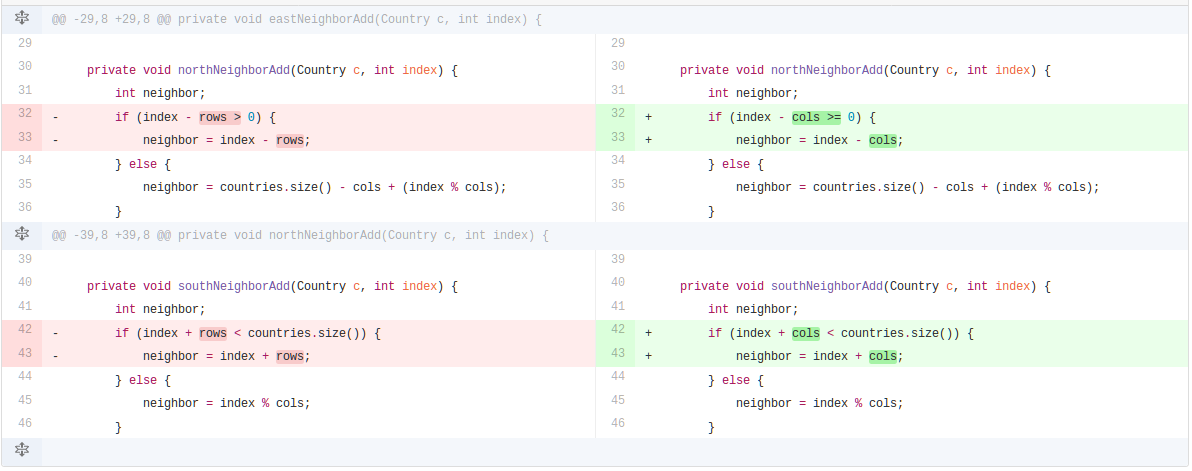
\includegraphics{./doc/index.png}
\caption{Neighbor Index Calculation Bug}
\end{figure}

Different map sizes weren't tested so ``rows'' related ``cols'' bug in
neighbor association was caught late.

\subsection{Countries Neighboring
Themselves}\label{countries-neighboring-themselves}

\begin{figure}[H]
\centering
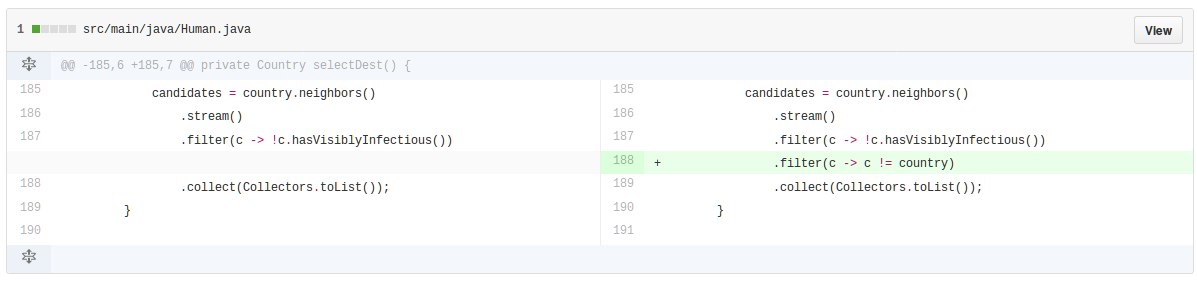
\includegraphics{doc/move.png}
\caption{Countries Neighboring Themselves}
\end{figure}

If countries were neighboring themselves due to round world rules, Human
objects considered their own country a move candidate. In this case they
were added to their population lists multiple times breaking the
population calculations.

\subsection{Dead Doctors Still
Vaccinating}\label{dead-doctors-still-vaccinating}

\begin{figure}[H]
\centering
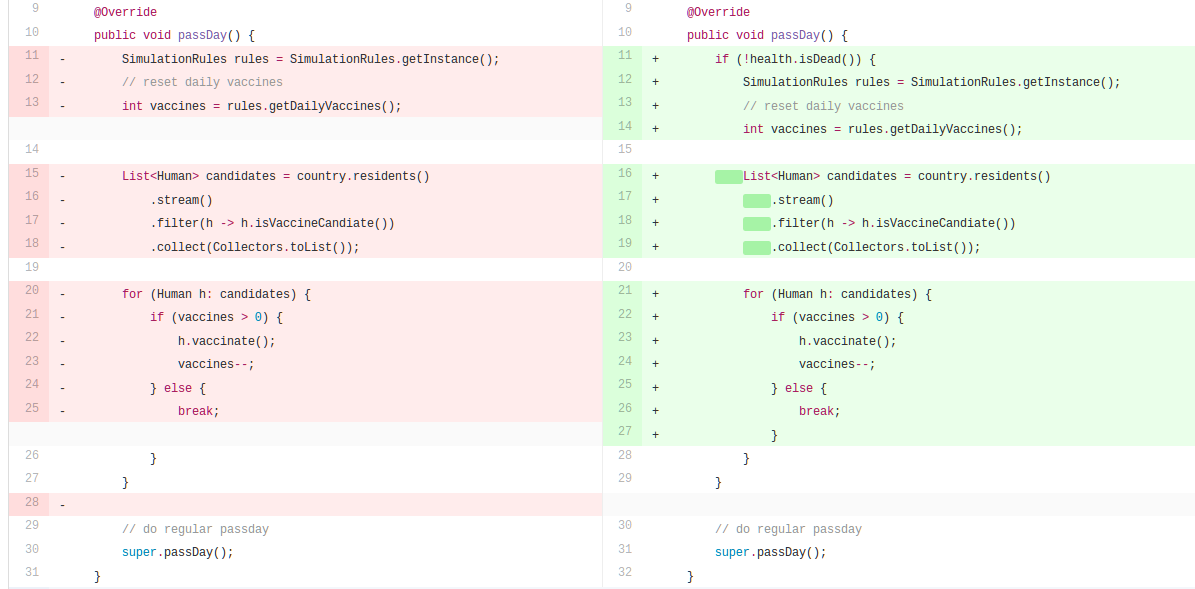
\includegraphics{doc/deaddoctor.png}
\caption{Dead Doctors Still Vaccinating}
\end{figure}

HealthState and Human's passDay actions unrelated to the health state
are kept separate. So it was easy to miss Dead state check for Doctor as
it was doing vaccination in it's own passDay and then just calling
\texttt{super.passDay()}.

\end{document}
